\documentclass[a4paper]{article}
\usepackage{amsmath}
\usepackage{graphicx}
\usepackage{url}

\title{Member 2 Report Draft}
\author{}
\date{}

\begin{document}
\maketitle

% ============================================================
% 2.2  Style Transfer and AdaIN
% Place in Related Works.
% ============================================================
\section{Style Transfer and AdaIN}

Neural style transfer separates the content of an image from its style. Gatys et al.\ define content as the spatial arrangement of higher-layer convolutional features, and style as correlation statistics across feature maps. Their method optimizes each content-style pair separately \cite{gatys2016image}. A new content image or a new style image requires a new optimization, so the method is not practical for making one augmented sample for each of the 1,349 Photo training images.

Later feed-forward methods replace that optimization with one network pass. Instance normalization subtracts each channel's own mean and divides by that channel's standard deviation, which reduces the contrast particular to the content image \cite{ulyanov2016instance,ulyanov2017improved}. AdaIN then replaces the content mean and standard deviation with those of the style image \cite{huang2017adain}. Let $f_c$ be the content features and $f_s$ the style features. For each channel, $\mu$ and $\sigma$ are the mean and standard deviation over all spatial locations:
\begin{equation}
\operatorname{AdaIN}(f_c,f_s)
=
\sigma(f_s)\odot\frac{f_c-\mu(f_c)}{\sigma(f_c)}+\mu(f_s).
\end{equation}
After this replacement, color and contrast come from the style image, while the spatial layout still comes from the content image. Any style image can be used at test time, without training a separate network for each style.

In this project the encoder is a fixed VGG-19, and its output is taken at relu4\_1. A decoder turns the features back into an image. The style strength $\alpha$ is a number between 0 and 1:
\begin{equation}
t=\alpha\cdot\operatorname{AdaIN}(f_c,f_s)+(1-\alpha)\cdot f_c.
\end{equation}
When $\alpha$ is 1, $t$ is the AdaIN output. This module uses pretrained encoder and decoder weights and does not train a new style-transfer network. The four prepared strengths are 0.25, 0.5, 0.75, and 1.0. The main comparison uses 1.0.

% ============================================================
% 2.3  Style Augmentation for Image Classification
% Place in Related Works. The PACS split belongs in Sections 2.1 and 3.2.
% ============================================================
\section{Style Augmentation for Image Classification}

The same object category can appear with different texture, brush strokes, and contrast in photos, paintings, cartoons, and sketches. Convolutional networks often rely on texture \cite{geirhos2019imagenet}. Changing appearance during training, while keeping the original class label, lets the classifier see the same category under more styles.

Jackson et al.\ sample a random style vector during training. The sampled style changes texture, contrast, and color, while the class label remains that of the content image \cite{jackson2019style}. Zhou et al.\ do not synthesize a new image in MixStyle. They mix the channel mean and variance of two training samples in feature space \cite{zhou2021mixstyle}. Those statistics are the same ones used by AdaIN. The mixing weight comes from a Beta distribution, and the style comes from the current training batch. The AdaIN augmentation in this project uses paintings from outside the training set and keeps an image that can be inspected one by one.

Content images come only from the PACS Photo training set \cite{li2017deeper}. Each stylized image keeps the original class and is then trained together with the original photo. The question is whether these new images raise accuracy on Art, Cartoon, and Sketch. Plain AdaIN uses one strength for the whole image. The main comparison uses 1.0. The other three values, 0.25, 0.5, and 0.75, are used to observe the effect of strength. The method that changes strength at each location according to image structure is written in the structure-preserving section. Both methods use the same content images and the same style images.

% ============================================================
% 3.4  AdaIN Style Augmentation
% Place in Methodology.
% ============================================================
\section{AdaIN Style Augmentation}

The three training settings share the same content images, the same style pool, and the same content-style pairs. The first setting uses the original Photo images only. The second adds the stylized images from this section. The third adds the structure-preserving stylized images. The main comparison for the second setting uses $\alpha=1$.

The content list is \texttt{project\_splits/photo\_train.txt}, with 1,349 images. Labels in the list run from 1 to 7. The data loader subtracts 1, so the labels used by the model run from 0 to 6. Style images are the 10 external paintings in \texttt{style\_pool/}, taken from the official PyTorch AdaIN examples.\footnote{\url{https://github.com/naoto0804/pytorch-AdaIN}} Their source is the same WikiArt line used by the AdaIN paper \cite{huang2017adain}. Content images remain PACS Photo images. The pool excludes \texttt{sketch.png}, which is close to the Sketch test domain, and it does not use PACS Art, Cartoon, or Sketch images. The Photo validation set, the Photo test set, and the three cross-domain test sets are not stylized and are not used to choose generation settings.

Pairs are fixed by seed 42. The 10 style images are shuffled with that seed. Content image $i$ receives the style at position $i \bmod 10$ in the shuffled list. Each training photo is paired with one style image. Repeating the run gives the same pairs, and all 10 styles are used.

Each pair is processed as follows.
\begin{enumerate}
  \item Convert the image to RGB and scale pixel values to the range 0 to 1. When the image is read from a file, resize its shorter side to 512.
  \item Encode both images to relu4\_1 with a frozen VGG-19, producing $f_c$ and $f_s$. The weight file is \texttt{models/vgg\_normalised.pth}.
  \item Compute the per-channel mean and standard deviation, and align them with the AdaIN formula above. The value $10^{-5}$ is added inside the standard deviation so that the denominator is not zero.
  \item Blend the features with the alpha formula above. The main comparison uses $\alpha=1$. The four strengths 0.25, 0.5, 0.75, and 1.0 are used for the strength comparison.
  \item Decode the features to RGB with a frozen decoder and clip the result to the range 0 to 1. The weight file is \texttt{models/decoder.pth}.
\end{enumerate}

A single image is produced by \texttt{stylize(content, style, alpha)}. To vary strength by location, call \texttt{encode}, \texttt{mix}, and \texttt{decode} in that order. \texttt{mix} accepts either one number or a strength map. The map is resized to the height and width of the feature map, and the blend at each location is
\begin{equation}
t(x,y)
=
\alpha(x,y)\cdot\operatorname{AdaIN}(f_c,f_s)(x,y)
+
\bigl(1-\alpha(x,y)\bigr)\cdot f_c(x,y).
\end{equation}
If the structure-preserving section uses $\alpha(x,y)=\alpha\bigl(1-\beta M(x,y)\bigr)$, that map is passed to \texttt{mix}. The content images, style images, pairs, and output size stay the same.

When only $\alpha=1$ is generated, images are written to \texttt{data/aug\_adain/images/} with the same relative paths as the original Photo images. When all four strengths are generated, they are written separately to \texttt{alpha\_0.25}, \texttt{alpha\_0.50}, \texttt{alpha\_0.75}, and \texttt{alpha\_1.00}. List labels remain the original values from 1 to 7. The main comparison trains on the original 1,349 images plus the 1,349 images at $\alpha=1$, which is 2,698 images in total. The structure-preserving setting uses the same 1,349 pairs.

What is finished now is a preview of the first 8 training photos at the four strengths, 32 images in total. These 32 images are for visual checking only. They are not added to the training set. The full set of 1,349 images has not been generated.

\begin{figure}[htbp]
  \centering
  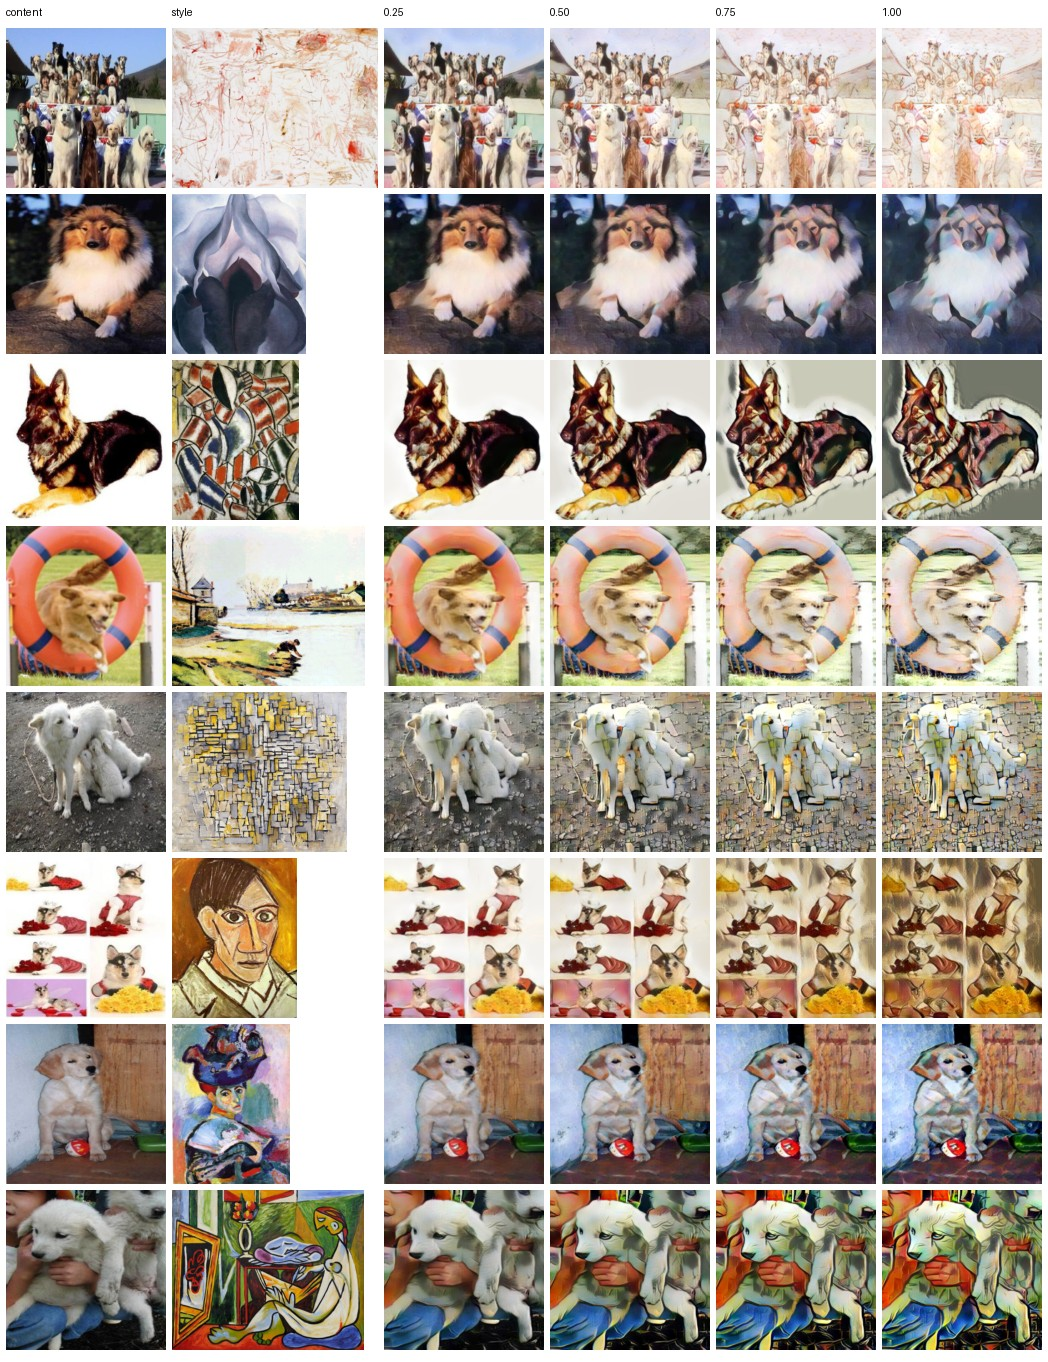
\includegraphics[width=\textwidth]{data/aug_adain/samples/alpha_overview.jpg}
  \caption{Preview of the first eight Photo training images. Each row shows, from left to right, the original image, the style image, and the results at strengths 0.25, 0.50, 0.75, and 1.00.}
\end{figure}

% ============================================================
% 4.2  AdaIN Augmentation Progress
% For Member 5 to merge into the progress section.
% ============================================================
\section{AdaIN Augmentation Progress}

\begin{enumerate}
  \item AdaIN inference is fixed. The encoder and decoder use public weights and are not updated during classifier training. The call is \texttt{stylize(content, style, alpha)}. \texttt{encode}, \texttt{mix}, and \texttt{decode} are available to Member 3, and a spatial strength map can be passed to \texttt{mix}.
  \item The style pool is fixed at 10 paintings outside PACS. Seed 42 assigns one style image to each of the 1,349 Photo training images. Art, Cartoon, Sketch, and the Photo validation and test sets are not stylized. The four strengths are 0.25, 0.5, 0.75, and 1.0. The main comparison uses 1.0.
  \item The flowchart is \texttt{figures/adain\_flowchart.svg}. Four-strength previews of the first 8 content images are in \texttt{data/aug\_adain/samples/}: 32 results, the matching side-by-side comparisons, and one overview. The full set of 1,349 images has not been generated. The script is \texttt{build\_adain\_aug.py}.
\end{enumerate}

\bibliographystyle{plain}
\bibliography{refs}

\end{document}
